\chapter{Action-angle variables in more detail}




\section{Poisson bracket of canonical coordinates}

\textbf{Definition:} Canonical coordinates are the ones which obey Hamilton's equations. \\
\textbf{Theorem:}  Any general canonical coordinates $(\vec{r}, \vec{p})$
 have the following PBs.
\begin{align}
\left\{p_{i}, p_{j}\right\}=\left\{r_{i}, r_{j}\right\}=0, 
&&\left\{r_{i}, p_{j}\right\}=\delta_{ij}.      \label{canonical_coordinates}
\end{align}
Also, any set of coordinates obeying the above PBs are canonical coordinates.




\hfill \break


\begin{definition}[label=def:CC]
See Theorem 10.17 of Ref.~\cite{fasano} for a proof of the above statement.
\end{definition}

\hfill \break





\section{Constructing action-angle variables}   \label{construct_AA}


In this section we will try to form a strategy to construct
 the action-angle coordinates
which satisfy the definition given in Sec.~\ref{define_integrable_sys}.
The definition of action-angle variables necessitates that the 
action-angle variables satisfy Eqs.~\ref{canonical_coordinates}.
We will break down our process of forming this strategy 
of constructing action-angle variables into a few steps. \\



\textbf{Step 1:} 


\textbf{Theorem:} Consider the following integral
\begin{align}
\mc{J}_i  =   \frac{1}{2 \pi} \oint_{\gamma_i}   \vv{P} \cdot  d\vv{Q},       \label{action_integral}
\end{align}
where the line integral is done over 
a loop $\gamma_i$ which is on the 
$n$-dimensional sub-manifold
defined by the constant values of the $n$ commuting constants.
The flow under $\mc{J}$ by an amount $2 \pi$ forms another closed loop
in the phase space on the  above mentioned $n$-dimensional sub-manifold.



See Definition 11.6 and Theorem 11.6 of
Ref.~\cite{fasano} for a proof of this statement.
This is pictorially shown in
Fig.~\ref{action_loop}. 
We will argue later that this integral
is the action variable.
Many textbooks take this expression of action as a definition \cite{goldstein2013classical}. \\






\begin{figure}
  \centering
  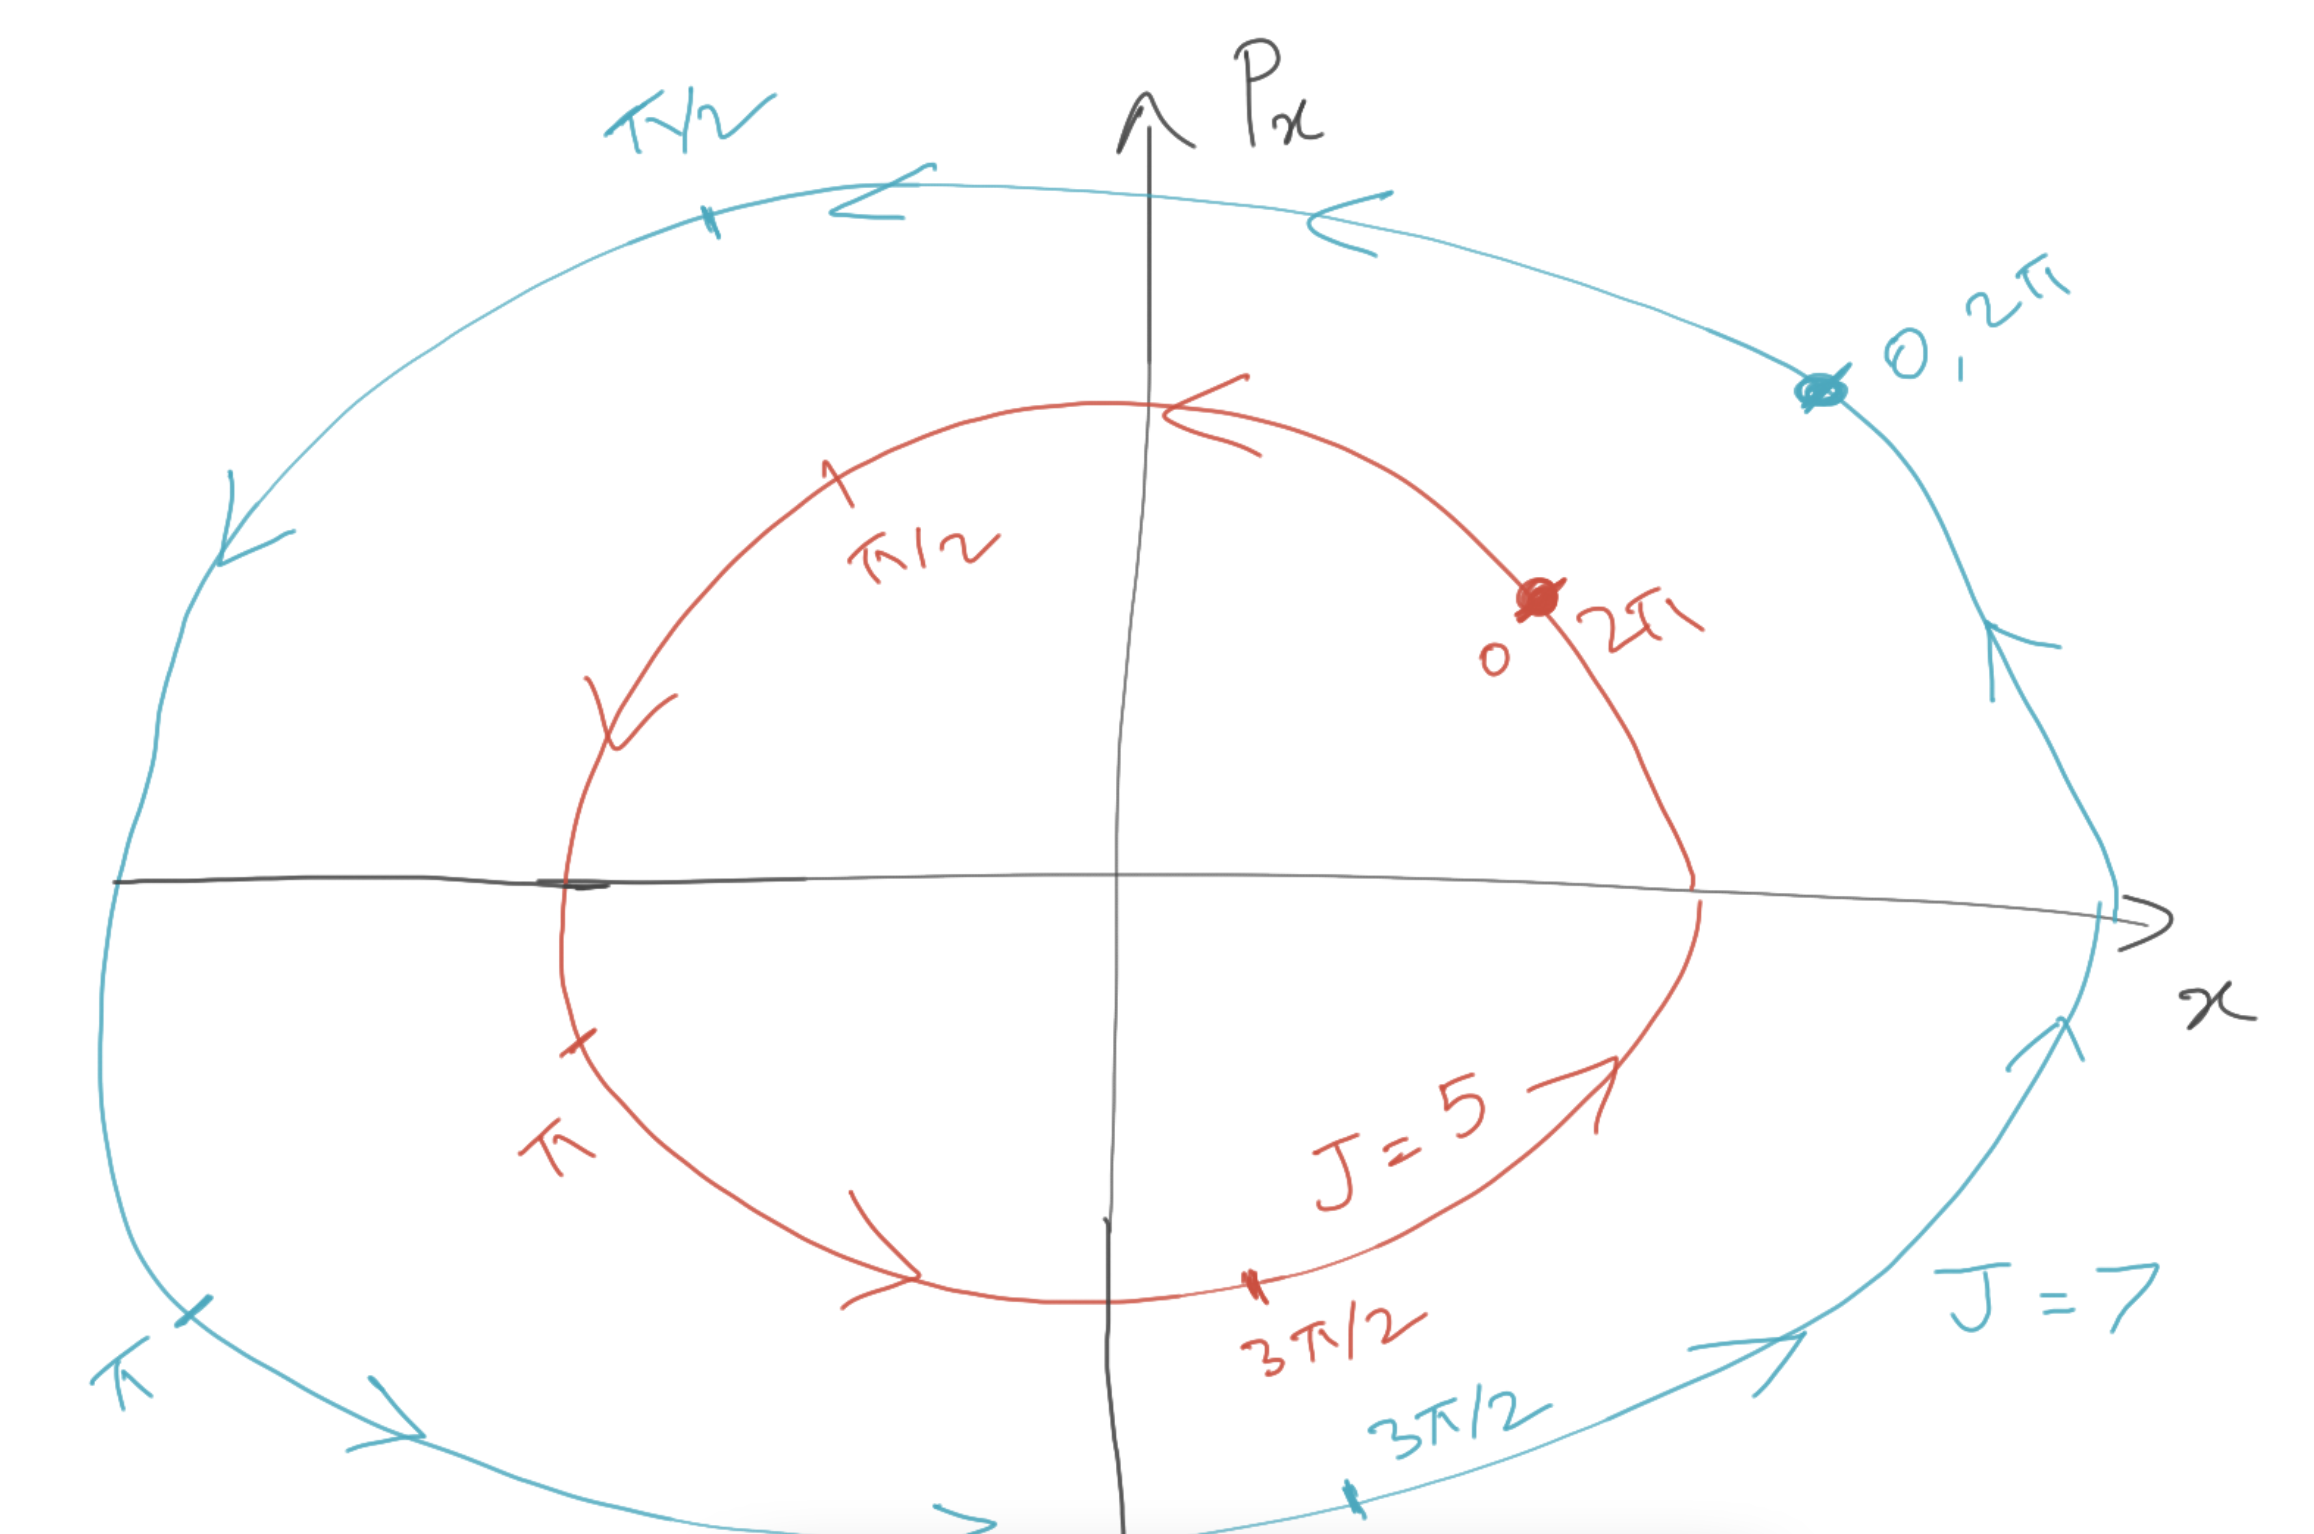
\includegraphics[width=0.7\linewidth]{action_loop}
  \caption{ Action flow makes a loop. On this loop,
  stamp the angle coordinates via $d \theta_i = d \lambda_i$,
  where $\lambda_i$ corresponds to the flow parameter under the 
  $\mc{J}_i$.
    \vspace{-1.em}
  }
  \label{action_loop}
\end{figure}





\hfill \break


\begin{definition}[label=def:C2]


Note that there are two different loops in the picture in the  
above discussions. The first is the $\gamma_i$ loop (Loop 1) over which
the action integral is evaluated, and the other is the one which is generated
by flowing under the action (Loop 2).\\


In general, these two loops are not the same.
Just like Loop 1,
Loop 2 is also in the $n$-dimensional submanifold
defined by the constants values of $C_i$'s, since
an action flow does not change the values of the $C_i$'s.
 Also, it can be shown that the action
integral evaluated on both the loops is the same.
 



\end{definition}

\hfill \break

\newpage


\textbf{Step 2:} 

\textbf{Theorem:} The $\mc{J}_i$ constructed above are mutually commuting, 
\begin{equation}
\left\{J_{i}, J_{k}\right\}  =  0.          \label{actions_commute}
\end{equation}


\textbf{Proof:}  
Let's denote by $\vec{C}$, the vector of all $n$ commuting constants.
Now all the $\mc{J}_i$'s can be considered to be functions of only the $C_i$'s,
(apart from some other constants like the masses of the BHs).
See the proof of Proposition 11.2 of Ref.~\cite{fasano} for a proof
of this statement.

If that is so then it follows that
\begin{equation}
\left\{J_{i}, J_{k}\right\}=\sum_{l, m=1}^{n} \frac{\partial J_{i}}{\partial C_{l}} \frac{\partial J_{k}}{\partial C_{m}}\left\{C_{l}, C_{m}\right\}=0 . 
\end{equation}
In the above proof, we have used the chain rule for PBs (introduced in
Eq.~\eqref{C0-PBs_defined_2}). So, we have succeeded in ensuring the first equality of Eqs.~\eqref{canonical_coordinates}
to hold true. (with $\vv{p} = \vv{\mc{J}}$). We now move on to ensure the last equality of 
Eqs.~\eqref{canonical_coordinates} holds true. We are talking about i.e. $\left\{r_{i}, p_{j}\right\}=\delta_{ij} $,
or rather $\left\{\theta_{i}, \mc{J}_{j}\right\} = \delta_{ij}$.   \\




\textbf{Step 3:} Construct the angle coordinates $\theta_i$'s the following way.
Dictate that the way to increase the angle $\theta_i$ (associated to $\mc{J}_i$
via $\pb{\theta_i, \mc{J}_j} = \delta_{ij}$),
and keeping other (action-angle) coordinates fixed
is to flow under $\mc{J}_i$, thus tracing a loop.
Also, demand that under this flow, $d \theta_i = d \lambda$.



Now, is this construction consistent with the action-angle 
PB $\pb{\theta_i, \mc{J}_j} = \delta_{ij}$?
Yes. To see this, let $f = \mc{J}_i$ and $\vv{V}$ be $\theta_i$
 in Eq.~\eqref{C2-H-flow}, which then becomes
\begin{align}
\frac{d \theta_i  }{d \lambda}   = \pb{  \theta_i ,  \mc{J}_i}  = 1  .  
\end{align}
Note that we equated the two quantities to $1$
because of our demand $d \theta_i = d \lambda$.
Under the same flow of $\mc{J}_i$, we also have 
\begin{align}
\frac{d V  }{d \lambda}   = 0  ,      
\end{align}
where $V$ stands for any of the action variables or any of the
angle variables (except for $\theta_i$). This is
because of Eq.~\eqref{actions_commute} and also the fact that
we dictated that
one and only one angle $\theta^i$ will change as we flow under $\mc{J}_i$.
Note that this way of construction of angle coordinates 
applies only on the $n$-dimensional submanifold defined by the constant
values of the commuting constants. We have not specified 
how to construct angle coordinates off this submanifold.
Thus, the last equality of Eq.~\eqref{canonical_coordinates} is ensured 
by our construction of angle coordinates.\\




\textbf{Step 4:} We won't try to ensure the second equality of 
Eq.~\eqref{canonical_coordinates}, i.e. 
$\pb{ \theta_i, \theta_j} = 0$, because flow 
under any of the $\theta_i$'s
implies changing the corresponding action 
($\theta_i,  \mc{J}_j = \delta_{ij}$),
and for real-time evolution (flow under the Hamiltonian), actions 
do not change (see Eq.~\eqref{C1-AA_eqn_1}). So there is not much use
in stamping the angle coordinates off the 
$n$-dimensional submanifold defined by the constant values of the 
actions or the commuting constants.\\



 


\textbf{Step 5:} One might worry that we can have infinite number of 
$\mc{J}_i$' since we can have infinite number of loops $\gamma_i$'s
over which the integral in Eq.~\eqref{action_integral} is to be
performed. This is in conflict with our expectation that the number of 
actions and angles both has to be $n$, so that $n+n = 2n$ is the
dimensionality of the phase-space. 



Actually, this is not a cause of concern. No matter how many action
integrals we compute using however many loops $\gamma_i$'s, there
will be only $n$ independent action variables. The rest will be linear 
combinations of these $n$ independent action variables. 
See Proposition 11.2 and 11.3 of Ref.~\cite{fasano} for a proof of this.\\



\textbf{Step 6:}
Now let's try to see if the action-angle variables defined or constructed
above match with the original definition given in Sec.~\ref{C1-definition}
or not. We will again not work things out from scratch but rather
outline the steps while referring to other sources.


We have already mentioned that
all the $\mc{J}_i$'s can be considered to be functions of only the $C_i$'s,
(apart from some other constants like the masses of the BHs).
All the $C_i$'s can also be considered to be functions of the
$\mc{J}_i$'s, i.e. $\mc{J}_i(\vec{C})$ is an invertible function,
if the determinant of the Jacobian of transformation 
(via the inverse function theorem)
is non-zero
\begin{align}
\operatorname{det}\left(\frac{\partial J_{i}}{\partial C_{j}}\right) \neq 0 .  \label{invert_condition}
\end{align}
The determinant is indeed non-zero for usual 
configurations. Now all this 
implies that the Hamiltonian (one of the $C_i$'s) is a function of
only the actions (in usual circumstances). This is
one of the defining criteria of action variables
(as per the definition given in Sec.~\ref{C1-definition}).





\hfill \break


\begin{definition}[label=def:C3]

\begin{center}
\textbf{Inverse of a function}
\end{center}

There needs to be some clarification in the context of 
the meaning of the $\mc{J}_i$'s being functions of $C_j$'s, 
and vice-versa. To simplify matters, lets talk in terms of 
a function $f$ of  a single variable $g$.\\


Note that $f$ being  a function of $g$ in the neighborhood
of point $g=g_0$ does not imply that 
$f$ has to be expressible in terms of $g$ in closed-form
using standard functions like sine, cosine, exponential or elliptic functions.
$f$ being  a function of $g$ in the neighborhood
of point $g=g_0$ means is that the function
$g(f)$ is an injective function in this neighborhood, so that
the inverse $f(g)$ is clearly defined. It may take numerical
root-finding to evaluate $f(g)$ but that's alright. 
See articles on implicit function theorem and inverse 
function theorem for more details. \\



For example, with the famous Kepler equation $l = u - e \sin u$,
$l$ is a function of $u$ (clearly), but $u$ is also a function of $l$
for all $l$'s since $l(u)$ is an injective function. Also, 
to evaluate $u(l)$, numerical root-finding is required. \\


Yet another example is $y= \sin x$, which does not have an inverse function
in a neighborhood around $x= \pi/2$ because in this neighborhood, 
$y(x)$ is not injective due to the maxima at $x= \pi/2$. So, one can't 
define $x(y)$ in this neighborhood, although one can clearly define 
$x(y)$ in small neighborhood around some other point say $x = \pi/4$.\\


So, for a one variable function $y(x)$,
 the inverse function does not exist in a 
neighborhood containing  a point $x_0$, where $dy/dx(x=x_0) = 0$. The 
generalization of this to multi-variable case is that the determinant
of the corresponding Jacobian has to be non-zero for the multi-variable
functions to be invertible (the inverse function theorem).
We apply precisely this theorem in Eq.~\eqref{invert_condition}.


\end{definition}

\hfill \break



Now let's come to the other criterion of this definition of action-angle variables.
The other criterion demands that 
{$\{ \vec{p}, \vec{q} \}(\theta_i + 2 \pi)  = \{ \vec{p}, \vec{q} \}(\theta_i ) $},
i.e. $\vv{p}$ and $\vv{q}$ are $2 \pi$-periodic
functions of $\theta_i$'s. This is clearly obvious from our construction of angle 
variables. As per this construction, changing only one of the angles
is tantamount to flowing under the corresponding action and doing so by an
amount $2 \pi$ brings us back to where we started from, thus forming  a loop. 
Hence, {$\{ \vec{p}, \vec{q} \}(\theta_i + 2 \pi)  = \{ \vec{p}, \vec{q} \}(\theta_i ) $} is indeed satisfied.





All in all, the take-home message is that (also shown in Fig.~\ref{action_loop})\\
\begin{tcolorbox}
as we flow under $\mc{J}_i$ (one of the actions), we form a loop after flowing by $\Delta \lambda_i = 2 \pi$.
We can also stamp the angle coordinate $\theta^i$ on this loop by setting $\theta_i = \lambda_i + C_0$, where 
$C_0$ is some constant real offset.
\end{tcolorbox}




\section{Action-angle variables of a simple harmonic oscillator}


Without explicit calculations, we state that for a SHO, the action-angle
variables are (with $\omega_0 =  \sqrt{k/m}$ and $\theta_0 \in \mathbb{R}$)
\begin{align}
\mc{J}  &= \frac{H}{\omega_0}  ,   \\
\theta    & = \arctan \frac{m \omega_0 q}{p} + \theta_0  .
\end{align}
The corresponding figure is again Fig.~\ref{action_loop}. Larger action
values means larger energy $H$ and hence a larger loop in the phase-space,
as is evident from the figure.





\section{How to flow under the actions?}






\begin{figure}
  \centering
  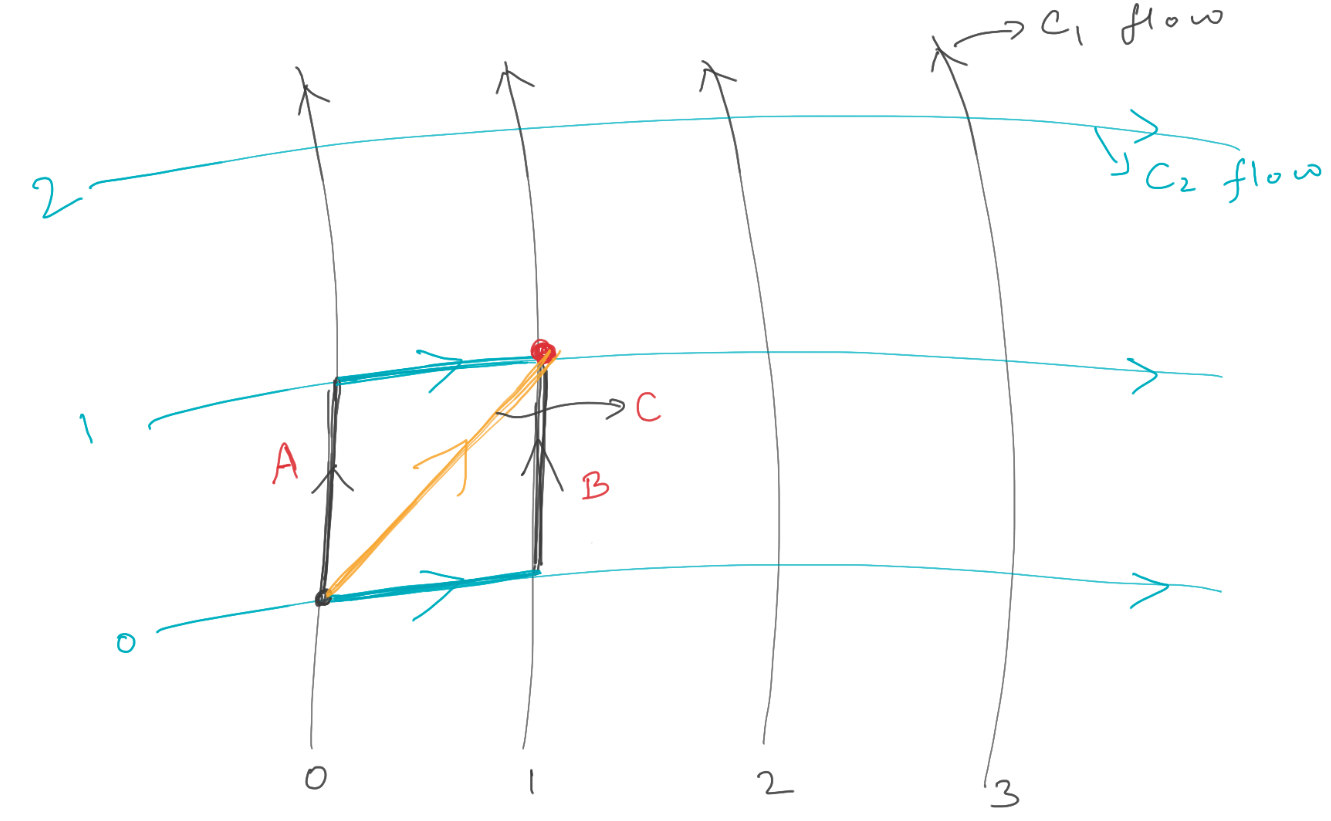
\includegraphics[width=0.8\linewidth]{flow_coordinates}
  \caption{ Setting up coordinates on the manifold using
  the flows of the commuting constants.
    \vspace{-1.em}
  }
  \label{flow_coordinates}
\end{figure}



\subsection{Flowing under commuting constants}    \label{flow_breakdown}

From Secs.~2.15 and 2.16 of Ref.~\cite{schutz1980geometrical},
or Sec.~9.6 and Exercise 9.9 of Ref.~\cite{misner2017gravitation},
we learn that vector fields of commuting quantities can be used to
set up coordinates on the manifold,
the flow parameter being the coordinate. We have already seen 
the application of this above
when we set up the angle coordinates along the flow of the
corresponding actions in Sec.~\ref{construct_AA}. 
Fig.~\ref{flow_coordinates}
is a pictorial depiction of setting up coordinates this way.



Now we state two theorems:
\begin{itemize}
\item \textbf{Theorem:} Order of flow under two commuting quantities
(need not be constants) does not matter.


Pictorially, flowing under two commuting quantities $C_1$ and $C_2$ 
in Fig.~\ref{flow_coordinates}
by fixed amounts in different orders (paths $A$ and $B$) 
starting from the same point 
point (black dot) leads us to the same ending point (red dot).




If we take for granted that vector fields of commuting 
quantities can be used to
set up coordinates on the manifold, with the 
flow parameter being the coordinate (see the 
beginning of Sec.~\ref{flow_breakdown}),
then the proof of this theorem
becomes almost self-evident from Fig.~\ref{flow_coordinates}.


\item \textbf{Theorem:} If $\pb{C_1, C_2} = 0$, then a flow under 
$C_1 + C_2$ by a certain amount $\Delta \lambda$ is equivalent 
to a flow under one of them followed by the other, each by an amount
$\Delta \lambda$.


Here is the proof. Let $\vec{V}^i$ denote one of the 
components of $\vec{R}, \vec{P}, \vec{S}_1$ and $\vec{S}_2$. Let
$\lambda_1$ and $\lambda_2$ denote the coordinates generated $C_1$
and $C_2$ flows as shown in Fig.~\ref{flow_coordinates}. So, we have
$V^i = V^i(\lambda_1, \lambda_2)$ and from basic multivariable
calculus
\begin{align}
& dV^i    = \frac{\pd V^i}{\pd \lambda_1} d \lambda_1 + \frac{\pd V^i}{\pd \lambda_2}   d \lambda_2   ,\\
&  \frac{dV^i}{d \lambda}    = \frac{\pd V^i}{\pd \lambda_1} + \frac{\pd V^i}{\pd \lambda_2}     \quad \quad  \text{if~}d\lambda_1 = d \lambda_2 = d \lambda  ,  \\
& \frac{dV^i}{d \lambda}   =  \pb{V^i , C_1} +  \pb{V^i , C_2} = \pb{V^i , C_1 + C_2} ,
\\
\implies  &  \frac{\pd V^i}{\pd \lambda_1} d \lambda + \frac{\pd V^i}{\pd \lambda_2}   d \lambda   =    \pb{V^i , C_1 + C_2}  d \lambda  .    \label{simul_flow}
\end{align}
Now the LHS of the above equation denotes the change in going from the
black dot to the red dot in Fig.~\ref{flow_coordinates},
which can be accomplished by flowing under $C_1$ and $C_2$ in any order 
(as already discussed after stating the previous theorem above).
This, along with Eq.~\eqref{simul_flow} finally proves the current theorem.
\end{itemize}




So, what we have learned is that  \\
\begin{tcolorbox}
\begin{itemize}
\item The order of flows under commuting quantities does not matter.
\item A simultaneous flow under commuting quantities 
by $\Delta \lambda$ can be broken down into the individual flows under them (by an amount $\Delta \lambda$ each).
\end{itemize}
\end{tcolorbox}








\subsection{Breaking down the action flow}      \label{action_flow_breakdown}



\begin{tcolorbox}
Let us assume two things for the rest of the material in this chapter
\begin{itemize}
\item We have all the actions in terms of the 
commuting constants: $\vec{J}(\vec{C})$. 
We will compute $\vec{J}(\vec{C})$ in Chapters \ref{C4-chapter-5}
and \ref{C5-chapter-6}.
\item We have closed-form solution for the flows under all the commuting
constants $C_i$'s. We will find these solutions for some
of the commuting constants in Chapter \ref{C4-chapter-5}.
The solution of the flows under the Hamiltonian and $\Eff$ 
is given in Refs.~\cite{Cho:2019brd} and \cite{tanay2021action}, 
respectively.
\end{itemize}
\end{tcolorbox}




With the above two assumptions, how 
can we flow under an action?
The answer is the chain-rule property of the PBs 
(Eq.~\eqref{C0-PBs_defined_2}). So, we have
\begin{equation}     \label{action_flow_2}
\frac{d \vec{V}}{d \lambda}=\left\{\vec{V}, \mc{J}_{i}\right\}=\left\{\vec{V}, C_{j}\right\}\left(\frac{\partial \mc{J}_{i}}{\partial C_{j}}\right).
\end{equation}
If we have $\cJ(\vv{C})$, then the partial derivatives can be evaluated and
they are simply constants because they will be functions of the $C_i$'s.
Apart from that, if we have the solution for flow under all the commuting 
constants, then the solution of flow under any of the actions
can be easily had. Note that Eq.~\eqref{action_flow_2} is the
equation for simultaneous flow under multiple commuting constants.
But from Sec.~\ref{flow_breakdown}, we know that we can flow under 
all these commuting 
constants one-by-one (order doesn't matter) and get the solution
for the flow under $\mc{J}_i$ by any finite amount, provided 
the we have $\mc{J}(\vv{C})$ and flow solution under all the $C_i$'s.






\subsection{Computing frequencies}    \label{compute_freq}


How do we compute the frequencies $\omega_i = \pd H/\pd \mc{J}_i$ given 
$\mc{J}_i(\vec{C})$, the Hamiltonian $H$ being one of the $C_i$'s?
It's trivial to compute the Jacobian $\pd \mc{J}_i/\pd C_j$ using 
a computer algebra system as \textsc{Mathematica}. 


Now, the frequencies $\omega_i = \pd H/\pd \mc{J}_i$ are elements of the 
the Jacobian of the inverse transformation, i.e. 
$\pd C_i/\pd \mc{J}_j$. From the inverse function theorem, we know 
that the Jacobian of the inverse transformation is the matrix 
inverse of the Jacobian of the original transformation.




\section{Constructing the action-angle based solution of the spinning BBH system}


We intentionally keep this section abnormally succinct. For a more detailed
step-by-step explanation on how to operationally construct the action-angle-based
solution, the reader is referred to Sec. IV of \cite{next_paper}.




Assuming that we have $\vec{\mc{J}}(\vv{C})$, and the solution for flow under
all the $C_i$'s, we now explicate the operational way to construct the
action-angle based solution of the system. $\vv{V}$ represents the totality of
the variables contained in the vectors $\vec{R}, \vec{P}, \vec{S}_1$ and $\vec{S}_2$,
and $\vv{V}_0$ denotes its initial value at time $t=0$.
We take $\vv{V}_0$ to correspond to all the angles being 0.


Suppose the solution is required at  a later time $t$. So, we know that
all the angles have changed to $\Delta \theta_i = \omega_i t$. 
We can easily have the numerical value of $\Delta \theta_i$ because we 
can compute all the $\omega_i$'s (see Sec.~\ref{compute_freq}).
Remember from Step 3 of Sec.~\ref{construct_AA}
that $\Delta \theta_i$, the change in the angles can be achieved by flowing 
under the corresponding actions by an equal amount
$\Delta \lambda_i = \Delta \theta_i$. The order of action flows does not matter
since $\pb{\mc{J}_i, \mc{J}_j} = 0$. Now the problem is reduced to flowing 
under all the $\mc{J}_i$'s by specified amounts, which we have
already figured out how to do in Sec.~\ref{action_flow_breakdown}.





\section{Afterthoughts and the plan ahead}



Now, the only missing ingredients towards constructing closed-form solutions
to the system are the $\vec{\mc{J}}(\vv{C})$ expressions and
the solutions of the flows under all the $C_i$'s.
We won't discuss the solutions of the flows under all the $C_i$'s, 
except for referring the reader to the relevant sources.
\begin{itemize}
\item The solution of the flow under $J^2, L^2$, and $J_z$ is very simple;
all the four 3D vectors 
$\vv{R}, \vv{P}, \vv{S}_1$ and $\vv{S}_2$ 
keep their magnitudes fixed and 
rotate around some fixed vector at a constant rate, with the exception that
spins don't move at all under the $L^2$ flow. We will discuss this 
to some degree in Chapter~\ref{C4-chapter-5}.
\item The solution of the flow under the Hamiltonian is worked out in 
Ref.~\cite{Cho:2019brd}. This paper ignores the 1PN Hamiltonian terms
for succinctness.
The solution is contained in Eqs.~(3.13, 3.24, 3.32, 3.42, 3.43)
of Ref.~\cite{Cho:2019brd}.

But we have already incorporated the 1PN terms of the Hamiltonian 
and implemented the flow solutions for $\vec{S}_1$ and $\vec{S}_2$ in a \textsc{Mathematica} package \texttt{BBHpnToolkit} \cite{MMA1}.
 The calculations behind this package will be presented in 
detail in an upcoming manuscript \cite{next_paper}.



\item The solution of flow under $\SeffL$ is worked out in 
Ref.~\cite{tanay2021action}.
The solution is contained in Eqs.~(A39, A65, A75)
of Ref.~\cite{tanay2021action}. Ref.~\cite{tanay2021action}
 does not explicitly give the solution
of $\vec{S}_1$ but it can be had in the 
same manner as that for $\vec{L}$ (Eq.~A65).
Then we can have $\vec{S}_2 = \vec{J} - \vec{L} -\vec{S}_1$.
\end{itemize}
So, in the remainder of these lecture notes, our focus will be on the only
remaining task which is to obtain $\vv{\cJ}(\vec{C})$.







